% \Image{Capa do livro (; )}{PNLD2022-011-01.png}

% \Image{Ilustração do livro (n-1 Edições/Isabel Lee; n-1 Edições)}{PNLD2022-011-04.png}
% \Image{Ilustração do livro (n-1 Edições/Isabel Lee; n-1 Edições)}{PNLD2022-011-05.png}
% \Image{Ilustração do livro (n-1 Edições/Isabel Lee; n-1 Edições)}{PNLD2022-011-06.png}


\documentclass[11pt]{extarticle}
\usepackage{manualdoprofessor}
\usepackage{fichatecnica}
\usepackage{lipsum,media9}
\usepackage[justification=raggedright]{caption}
\usepackage[one]{bncc}
\usepackage[nmenosum]{../edlab}
\usepackage{marginnote}
\usepackage{pdfpages}
\usepackage[printwatermark]{xwatermark}
%\newwatermark[pagex=2]{
\includegraphics[scale=3.3]{watermarks/test-a.png}}	% página específica
%\newwatermark[oddpages]{
\includegraphics{watermarks/test-a.png}}			% páginas ímpars
%\newwatermark[evenpages]{
\includegraphics{watermarks/test-a.png}}			% págimas pares
\newwatermark[allpages]{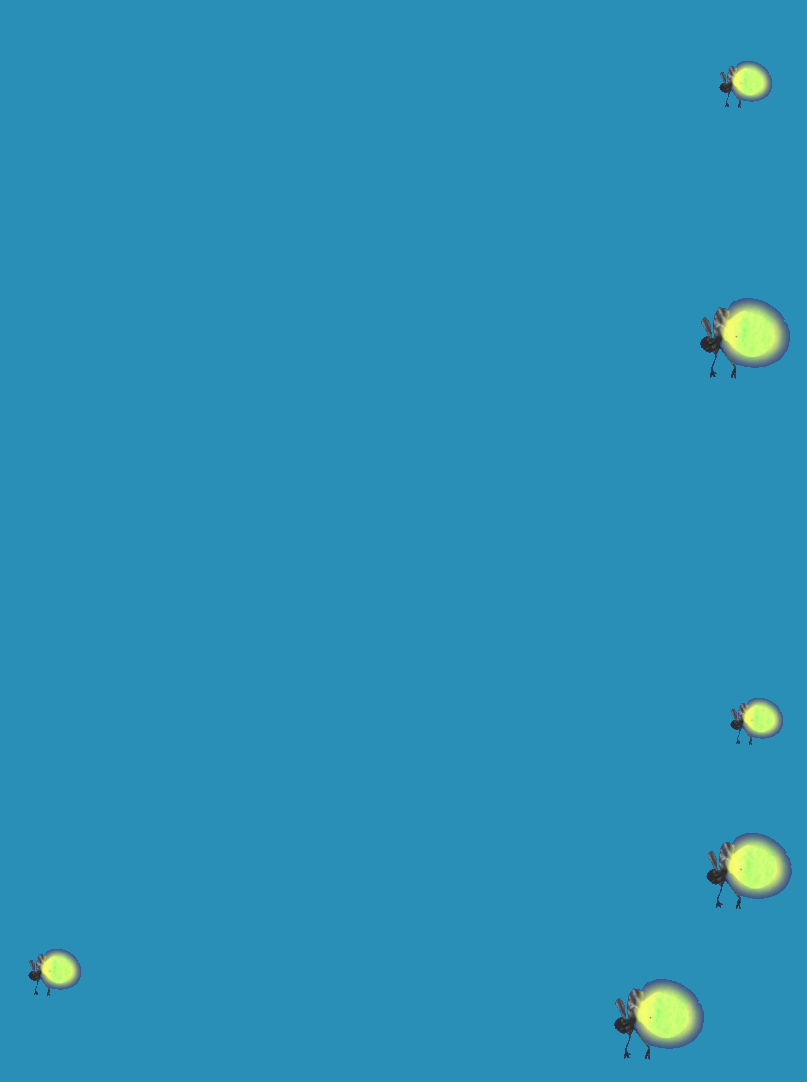
\includegraphics[scale=1]{watermarks/011.png}}

%\pagecolor{cyan!0!magenta!10!yellow!28!black!28!}

\newcommand{\AutorLivro}{Camila Werner}
\newcommand{\TituloLivro}{Calu e os animais}
\newcommand{\Tema}{Animais da fauna local; nacional e mundial}
\newcommand{\Genero}{Narrativos: fábulas originais; da literatura universal e da tradição popular; etc}
\newcommand{\imagemCapa}{./images/PNLD2022-011-01.png}
\newcommand{\issnppub}{978-65-86941-65-4}
\newcommand{\issnepub}{978-65-86941-67-8}
% \newcommand{\fichacatalografica}{PNLD0001-00.png}
\newcommand{\colaborador}{{Paulo Pompermaier e Renier Silva}}

\begin{document}

\title{\TituloLivro}
\author{\AutorLivro}
\def\authornotes{\colaborador}

\date{}
\maketitle

%\begin{abstract}\addcontentsline{toc}{section}{Carta ao professor}
%\pagebreak

\tableofcontents



\section{Sobre o livro}

%27 caracteres
\paragraph{O livro} 
``Calu e os animais'' é um livro com textos e ilustrações.
%822 caracteres
\paragraph{Descrição} 
A cada página de ``Calu e os animais'' são apresentados animais
que fazem parte do quotidiano das crianças brasileiras e outros
que podem ser encontrados numa visita ao zoológico. 
A cada novo animal são descobertas novas características que lhes
distinguem: uns têm boca, outros têm bico; uns nadam, outros voam;
uns são pequenos, outros são grandes. 
A aventura começa com os animais de casa, um gato e um cachorro.
Quando Calu vi ao zoológico, a criança conhece animais selvagens
como a onça-pintada, a zebra e o jacaré. 
No fim do dia, ao voltar para casa, os animais noturnos
dão as caras: a coruja e o vaga-lume fecham o livro com belas ilustrações.
%411 caracteres
\paragraph{Competências} 
São muitas as competências trabalhadas por este livro com os estudantes da \textbf{Pré-escola}.
A começar pela apreciação das pinturas que ilustram as páginas que são por si só uma
obra de arte. Com a apresentação dos animais da fauna nacional e do mundo, as crianças
terão garantido seu direito, descrito pela \textsc{bncc}, de explorar os elementos da natureza
e ampliar seus saberes sobre a cultura em suas diversas modalidades: artes, escrita e ciência.

%862 caracteres
\paragraph{Aprofundamento} 
Este material tem a intenção de contribuir para que você consiga desenvolver um trabalho aprofundado 
com esta obra na sala de aula. Você encontrará informações sobre o autor, sobre 
o gênero e sobre os temas trabalhados ao longo do livro. Apresentaremos também 
algumas propostas de trabalho para a sala de aula que você poderá explorar livremente, 
da forma que considerar mais apropriada para os seus estudantes. Para a prática 
da Literacia Familiar, oferecemos um guia que pode ajudar nas orientações aos 
responsáveis pela criança, para incentivar o gosto pela leitura e contribuir para 
que os estudantes desenvolvam em casa habilidades que serão importantes no momento 
da alfabetização. Por fim, você encontrará sugestões de livros, artigos e sites 
selecionados para enriquecer a sua experiência de leitura e, 
consequentemente, a de seus estudantes.

\reversemarginpar
\marginparwidth=5cm



\section{Sobre os autores}


%532 caracteres
\paragraph{A autora}
Atua há 18 anos no 
mercado editorial brasileiro e internacional, com experiência 
em diversos segmentos como didático, literatura, trade, 
referência, acadêmico e infantojuvenil, entre outros. 

\marginnote{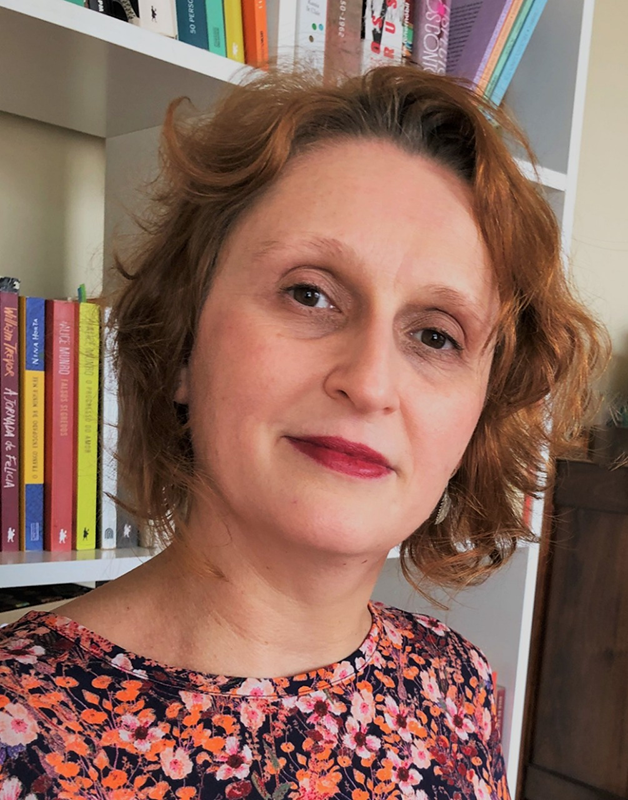
\includegraphics[width=\marginparwidth]{./images/PNLD2022-011-02.png}\\
A autora Camila Werner (Arquivo pessoal)\\\bigskip
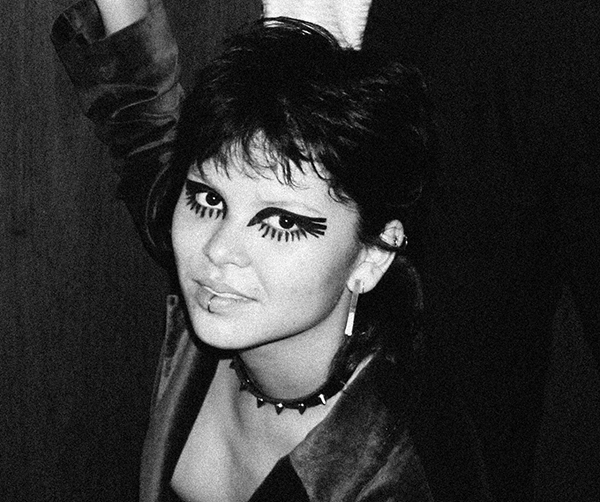
\includegraphics[width=\marginparwidth]{./images/PNLD2022-011-03.png}\\
A ilustradora Isabel Lee (Arquivo pessoal)}

%313 caracteres
\paragraph{Publicações}
Publicou pela editora Hedra os seguintes livros: \emph{Bolotas e quadrados},
\emph{Esconde-esconde}, \emph{Bom dia, Calu}, \emph{Na casa de Calu}, \emph{Calu e os animais} e
\emph{Calu e as frutas}, todos voltados para o público infantil.


%358 caracteres
\paragraph{Currículo} 
Formada em Comunicação Social com 
especialização em Produção Editorial pela \textsc{eca/usp} 
e mestrado em Books and Digital Media Studies pela 
Universidade de Leiden, Países Baixos.
Atualmente coordena o departamento digital da Brinque 
Book, editora especializada em livros infantojuvenis.




\section{Sobre o gênero}

%55 caracteres
\paragraph{O gênero} O gênero deste livro é \textit{narrativa}. 

%596 caracteres
\paragraph{Descrição} 
O gênero narrativo possui uma variedade de tipos e, cada um, suas estruturas específicas.
A característica comum entre todos é que sempre há uma história a ser contada, com linearidade,
ou seja, começo, meio e fim, e personagens. 
Dentre os tipos de narrativas mais comuns na literatura infantil, estão: mito, lenda, 
fábula e apólogo. Este último, semelhante à fábula, possui personagens não humanos, 
dramatização de fala, e uma moral, implícita ou explícita, mas difere na natureza destas 
personagens: se no caso da fábula se trata de animais, no caso do apólogo as personagens 
são objetos inanimados. No caso deste livro, a pinta de uma joaninha, que é mais um 
símbolo do que um objeto. Quase qualquer coisa pode ser uma personagem de uma narrativa 
infantil, já que a capacidade reflexiva das crianças nesta idade ainda está em um nível primário. 


%603 caracteres
\paragraph{Interação} 
As narrativas são uma forma de inserir os sujeitos no mundo. 
São elas que apresentam boa parte dos valores culturais da sociedade 
onde se vive. Mas não é só passivo o papel das crianças nesta experiência. 
As interações entre dois ou mais personagens onde se verifica
uma ação de linguagem organiza e impulsiona experiências compartilhadas,
importantes para o desenvolvimento psíquico do sujeito nos primeiros anos de vida.
Neste sentido, as narrativas são uma ótima ferramenta para
apresentar o mundo e capacitar as crianças para viver nele, mas como se
trata de um trabalho com a linguagem, sempre dando espaço à individualidade, 
seja na compreensão das histórias, na identificação com as personagens, ou 
no ato de narrar. 

\Image{O gênero da narrativa proporciona ao leitor uma abertura ao mundo. (Pixabay/Tumisu; CC-BY-2.0)}{PNLD2022-011-07.png}

%862 caracteres
\paragraph{Competências} 
A narrativa da ``Calu e os animais'' trabalha diferentes competências
nos pequenos leitores. Desde o começo o gênero narrativo sempre teve
a característica de apresentar novidades provindas de uma aventura.
A aventura, neste caso, é a descoberta da fauna nacional e mundial
por meio da observação dos bichos em um zoológico e no ambiente doméstico.
A criança aprende a perceber as diferenças entre os animais, os cuidados
e a natureza específica de cada um. Aprender sobre a diversidade
no mundo natural é um passo importante para se constituir em seu imaginário
a coexistência entre formas e seres vivos diferentes que convivem 
harmonicamente num mesmo lugar. O respeito à fauna por si só
será importante, além de refletir no respeito a si mesma e ao outro
no decorrer do desenvolvimento de sua individualidade. 

\section{Temas}

\subsection{Animais da fauna local; nacional e mundial}

%136 caracteres
\paragraph{Abordagem} 
Os animais da fauna local e mundial são apresentados no ambiente 
doméstico e numa viagem ao zoológico.
%206 caracteres
\paragraph{Descrição} 
A cada página, uma criança conhece as características físicas
e comportamentais de animais domésticos e selvagens apresentados
em comparação entre si. 
%275 caracteres
\paragraph{Competências} 
O tema tratado neste livro propõe a discussão de noções de espaço, 
de tempo, de quantidade, de relações e de transformações de elementos
do mundo natural, propondo motivar a criança a ter um olhar mais crítico
e criativo do mundo por meio de atividades significativas.

\section{Modelagem de aula}
A seguir você encontrará a descrição de uma aula modelo como exemplo 
prático de exploração do livro com estudantes. Esta seção apresentará 
orientações sobre como organizar a sala de aula para receber os 
estudantes, exercitar a interação verbal e prepará-los para o 
momento da leitura.

Em seguida, você encontrará a \textbf{Leitura dialogada}, um 
tópico destinado a te orientar para o momento específico da 
leitura com os estudantes. Por fim, no tópico 
\textbf{Propostas de atividades}, você encontrará ideias 
de práticas que pode explorar com as crianças em sala de 
aula após a leitura. 

Essas atividades podem ser trabalhadas de acordo com a 
disponibilidade do seu cronograma e fique à vontade para adaptá-las 
da forma que achar melhor para os seus estudantes. Cada turma é única 
e o seu conhecimento prático das características de cada aluno será 
essencial para definir a melhor forma de aplicar essas ideias. 

O objetivo deste manual é oferecer algumas ideias 
e inspirações para um trabalho que pode ser desenvolvido tanto 
a curto, quanto a médio e longo prazo. Sinta-se a vontade para 
personalizar a aula e torna-la sua, aplicando seus conhecimentos, sua 
personalidade e aproveite para fortalecer 
seu vínculo com a turma.


\subsection{Antes de ler}

\BNCC{EI02EO06} 
\BNCC{EI02EF03} 
\BNCC{EI02EF04} 
\BNCC{EI02EF06} 
\BNCC{EI02EF07} 
\BNCC{EI02EF08} 
\BNCC{EI02EF09}

%Alterar o nível escolar nesse parágrafo.
Como este trabalho será realizado com crianças da \textbf{Creche \textsc{ii}}, 
que ainda não têm muita intimidade com o livro enquanto objeto, você terá o 
papel de mediar este contato. 

Nosso objetivo é que os próprios estudantes possam manusear 
e explorar o livro de forma autônoma, mas, para que isto aconteça, você 
pode ajudar a tornar o caminho mais convidativo com atividades que tenham 
intencionalidade educativa. 

A \textsc{bncc} define intencionalidade educativa como ``organização 
e proposição, pelo educador, de experiências que permitam às crianças 
conhecer a si e ao outro e de conhecer e compreender as relações com a 
natureza, com a cultura e com a produção científica, que se traduzem nas 
práticas de cuidados pessoais (alimentar-se, vestir-se, higienizar-se), 
nas brincadeiras, nas experimentações com materiais 
variados, na aproximação com a literatura e no encontro com as 
pessoas''.\footnote{\textsc{bncc}, página 39}

É importante manter essa intencionalidade em mente não apenas na condução 
das atividades propostas neste manual, mas também para aproveitar as 
oportunidades espontâneas de construir conhecimentos que podem surgir durante 
a interação direta com os estudantes.

\begin{enumerate}
%836 caracteres
\item \textbf{O ambiente}\quad Antes de iniciar o trabalho com o livro, é importante que você 
prepare o ambiente para receber a turma. Como o trabalho com o livro terá 
três momentos (antes, durante e depois da leitura), seria interessante que você 
criasse um ambiente para cada etapa. Nas \textbf{Sugestões de referências complementares} 
você encontrará um artigo que discorre sobre a importância da organização da sala 
de aula para a educação infantil, que pode ser um bom guia para a criação desses 
ambientes. Para o momento antes da leitura, você pode decorar a sala com animais 
da fauna nacional e mundial na forma de fotos, pelúcias, fantoches, máscaras\dots{}
Também pode colocar como trilha sonora uma música com tema de floresta, com 
cantos de pássaros, por exemplo.

\Image{Exemplo de imagem de animais para decoração da sala. (Public domain pictures; Domínio público)}{PNLD2022-011-09.png}

%413 caracteres
\item \textbf{Primeira opção}\quad Utilize os primeiros 
momentos da aula para passear por essa área, chamando atenção para cada um 
dos animais e suas características. Pergunte-lhes os nomes, onde vivem,
se alguém já viu um pessoalmente\dots{} É importante que todas as contribuições 
sejam ouvidas. Repita alto para todos sempre que alguém falar. Estimule
o lúdico das crianças vestindo as máscaras do bichos e imitando os 
sons que eles fazem, então peça para que façam o mesmo.

\Image{Outro exemplo de imagem de animais para decoração da sala. (Pixabay; CC-BY-2.0)}{PNLD2022-011-10.png}


%632 caracteres
\item \textbf{Segunda opção}\quad Outra possibilidade para familiarizar 
as crianças com os animais que serão abordados no livro é dançar
com eles em meio às representações dos bichos. Para isso,
é importante que a música ambiente escolhida seja dançante
e divertida. Estimule os alunos a soltar seus corpos
e reagir com eles aos sons e ritmos. Não deixe de interagir
verbalmente com as crianças durante a dança.
Chame a atenção dos colegas para um novo movimento que uma
delas fizer. Elogie, pergunte se ela está imitando algum bicho e
peça que os colegas imitem o movimento.
\end{enumerate}


\subsubsection{A interação verbal} 
Criar situações em que as crianças precisam dialogar diretamente com 
você é uma das práticas mais importantes de Literacia, pois elas estimulam 
o desenvolvimento linguístico, ampliam o vocabulário e reforçam a 
capacidade dos estudantes de compreenderem o que ouvem e se expressarem 
pela fala. O diálogo livre com a criança também reforça sua autoestima, pois 
a faz se sentir ouvida e valorizada pelo adulto, ao vê-lo prestar atenção 
no que ela tem a dizer. Portanto, sempre que possível, reserve um tempo na 
aula apenas para a interação verbal. 

Como esse tipo de interação é espontânea e intimamente atrelada ao 
desenvolvimento de cada estudante, nossas orientações não serão específicas. 
A ideia é que você adapte este momento de acordo com as respostas e os 
repertórios das crianças. É um momento de estreitamento de vínculos e, portanto, 
fique a vontade para ser espontânea e para explorar os tópicos que achar 
mais interessantes para a sua turma.

Inicie as conversas com naturalidade, seguindo os objetos de atenção das crianças. 
Você pode partir de objetos que estejam analisando
para iniciar um assunto e incentivar a se expressarem. Ainda
que a criança não fale corretamente, continue interagindo, pois a
intenção aqui é que ela perceba que outras pessoas estão respondendo à sua comunicação.

Fique atento a todas as formas de expressão: os gestos, as falas, as 
expressões faciais, para onde olham\ldots{} tudo pode ser explorado durante a conversa. 
Demonstre curiosidade sobre eles, seja um ouvinte entusiasmado e incentive que eles 
conversem entre si. Faça perguntas e construa a resposta junto com as crianças. 

A seguir, algumas dicas que podem contribuir para que a interação verbal 
seja produtiva em sua sala de aula: 

\begin{enumerate}
\item Sente-se no chão e brinque com eles, estabelecendo 
contato visual. Além das pequenas frases que conseguem formar,
vocalizações, gestos e expressões faciais podem ser boas formas
de comunicar.

\item Não se esqueça de que a conversa é uma troca e, portanto, evite
ficar falando sozinho ou desvalorizar as respostas das crianças
quando não conseguem formular frases completamente
articuladas. Nunca descarte uma tentativa de comunicação.

\item Evite utilizar falas negativas que desencorajam o diálogo. 
Se precisar que a turma 
corrija algum comportamento, explique claramente a razão e 
oriente com calma. Incentive positivamente as crianças e 
destaque o motivo de seus elogios. 

\item Aproveite alguns momentos durante a conversa para chamar 
a atenção das crianças para os sons das palavras e das letras que você 
acabou de usar ou que eles pronunciaram.  

\item Explore possibilidades de interação como apontar e 
nomear objetos, pessoas e animais ou fazer caretas, reproduzir sons de 
animais para que repitam, ensinar os nomes de partes do corpo, 
entre outras atitudes que estimulem a comunicação com a criança. 

\item Muitas dessas dicas poderão ser aproveitadas pela 
família durante a prática da Literacia Familiar. Portanto, 
se achar necessário, compartilhe algumas destas orientações 
com as famílias dos estudantes.
\end{enumerate}


\subsection{A leitura dialogada}
Este é o momento em que será realizada a leitura propriamente dita. 
Se possível, crie um \textit{cantinho da leitura} em sua sala de aula. Um 
ambiente confortável, de preferência em que todos se sentem no chão ou 
em pufes para que consigam enxergar as ilustrações do livro que está 
sendo lido e interagir com facilidade. Se houver possibilidade, mantenha 
sempre os livros da turma em uma altura da estante que permita fácil 
acesso para os estudantes ou guarde os livros em uma caixa que as crianças 
possam mexer com autonomia. É importante que elas tenham autonomia para 
acessar os livros e se sintam à vontade para pegá-los sempre que quiserem. 

\Image{É importante que o cantinho da leitura proporcione autonomia para as crianças. (Elza Fiúza/ Agência Brasil; CC BY-NC 2.0)}{PNLD2022-011-08.png}

Outra possibilidade de ambiente para esta leitura, se a escola permitir, 
é efetuar essa leitura ao ar livre, embaixo de uma árvore, onde as crianças 
possam ouvir os sons dos pássaros e sentir o cheiro da grama. Sair da sala 
de aula pode oferecer um ótimo leque de experiências aos seus estudantes e 
reforçar a conexão entre a natureza do livro e a realidade.  

Reserve uma boa parte da aula para o momento da leitura com os estudantes, 
pois é importante que esse momento aconteça sem pressa. O objetivo da 
leitura dialogada é que seja uma leitura em bate-papo. A criança deve 
assumir um papel ativo na leitura, mesmo que ainda não seja capaz de 
ler sozinha. Além de promover o gosto pela leitura, esta prática estimula 
o desenvolvimento da linguagem, enriquece o vocabulário e 
aumenta o conhecimento de mundo.

%Especificar o livro.
No caso de “Calu e os animais” oo diálogo durante a leitura
é importante para verificar se as crianças estão acompanhando
a narrativa. As características de cada animal são dadas
também pela linguagem visual mas é o aparato descritivo do
texto é muito importante para estabelecer as diferenças
entre os bichos. Por isso, repita sempre as frases e palavras.

A seguir, algumas orientações para aproveitar este momento: 

\begin{enumerate}
%177 caracteres
\item \textbf{Como começar}\quad Sente-se em um lugar acessível, 
onde todos conseguirão ouvir bem a sua leitura e enxergar as ilustrações 
quando você estiver mostrando o livro ou eles estiverem manuseando-o. 
Antes de abrir o livro, chame a atenção dos estudantes para a capa. 
Faça perguntas sobre a capa, como: 

\begin{itemize}
\item Que bichinhos são esses?
\item Quem tem um gatinho em casa?
\item E quem tem um cachorro?
\item Qual o nome deles? E a cor?
\item Vocês conhecem o elefante?
\end{itemize}

Estas perguntas te ajudarão a avaliar repertório das crianças 
e fazê-las perceber que elas já conhecem os nomes de alguns animais. Se achar 
conveniente, peça que repitam algumas palavras com você e valorize tentativas 
de imitar a sua fala. 
 
%230 caracteres
\item \textbf{Manuseio}\quad Deixe que as crianças manuseiem o livro 
e explore com elas todos os elementos que o compõe. Mostre o que é a 
capa e onde estão as páginas. Leia o título do livro em voz alta, seguindo 
a leitura com o dedo, indicando as letras. 

%495 caracteres
\item \textbf{Diálogo}\quad A cada página ou a cada novo animal,
chame a atenção dos alunos para ele. Faça perguntas como:

\begin{itemize}
\item Quem já viu esse bicho?
\item Onde ele mora?
\item Ele sabe nadar? Ele voa? 
\end{itemize}

Se os estudantes não conseguirem responder, explique ou mostre uma 
imagem ou um vídeo. Traga referências além da ilustração e da frase. 
Incentive-os a imaginar coisas sobre os animais a partir da ilustração
e das descrições do livro.

\includepdf[nup=2x3, 				% grid
			%offset=-15mm -5mm, 	% posição
			scale=.8, 				% tamanho da página
            delta=4mm 4mm, 			
            frame,
            pages={4-5,8-9,16-17}]{./pdfs/\jobname_MIOLO.pdf}

%346 caracteres
\item \textbf{Escuta}\quad Elogie atitudes positivas, como 
tentar tomar o papel central na leitura. Se os estudantes tentarem 
tomar o seu lugar e começar a narrar a história --- com palavras já articuladas 
ou não --- valorize e escute com atenção o que estiverem falando. Mas não 
force a leitura. Se as crianças estiverem cansadas, faça outra atividade 
e retorne depois. 

%935 caracteres
\item \textbf{Leitura}\quad Durante a leitura você pode
perguntar aos alunos se eles conhecem os animais que estão ilustrados.
Como eles não são nomeados no texto, você pode apresentar os seus nomes.
Antes, no entanto, é interessante que você faça perguntas como:

\begin{itemize}
\item Que bicho é esse que voa e é colorido?
\item E esse que tem várias listras pretas e brancas?
\item E esse que mora no mar?
\end{itemize}

Não tenha pressa em passar as páginas. 
A intenção é que seja uma leitura com bastante comentários
da parte deles. Aproveite para dar mais detalhes sobre cada 
um dos bichos, como seu habitat, seus hábitos, onde podem ser
encontrados (perto da comunidade no caso dos mais acessíveis,
ou num zoológico, no caso dos naturais de outras regiões).
Crie um ambiente amigável onde a criança se sinta à vontade 
para fazer perguntas e comentários durante a leitura.


%382 caracteres
\item \textbf{Interação}\quad Nomeie os elementos das ilustrações 
do livro, apontando para elas com o dedo. Destaque os sons de algumas 
palavras. Interrompa a leitura em alguns momentos e peça que 
os estudantes repitam palavras, como \textit{zebra}, \textit{jacaré}, 
\textit{vaga-lume}. Se possível, leia a várias vezes, alterando a 
ordem de apresentação dos animais.
\end{enumerate}


\subsection{Propostas de atividades}

\BNCC{EI02CG05} 
\BNCC{EI02TS02} 
\BNCC{EI02EF03}

\begin{enumerate}
%700 caracteres
\item \textbf{Contexto}\quad Após a leitura dialogada, é hora de criar 
atividades que proporcionem aos estudantes experiências novas a partir da história 
que acabaram de conhecer. Nesta idade é fundamental explorar os sentidos da criança e 
ajudá-lo a experimentar a história que acabou de conhecer de formas diversas. Se achar 
conveniente, convide os estudantes a se sentarem nas carteiras para este terceiro 
momento, pois muitas atividades que serão realizadas exigem apoio para escrever 
ou manipular objetos. É interessante, por exemplo, que a criança perceba a conexão 
entre as imagens que acabou de ver e os elementos da realidade. Para ajudar a traçar 
essa relação, separe previamente objetos da natureza relacionados ao livro. 

\item \textbf{Materiais}\quad 
Massa de modelar de diversas cores.
%650 caracteres
\item \textbf{Ambiente}\quad  
Na sala de aula ou num espaço aberto. 

%950 caracteres
\item \textbf{A atividade}\quad Como os animais de “Calu e os animais” são
apresentados a partir de pinturas, você pode construir uma ponte interessante com as 
artes plásticas. Distribua as massinhas de cores diferentes para as crianças
e peça para elas criarem os animais ilustrados no livro que leram. 
Trabalhar com esse material pode ser muito produtivo pois, além de afinar o 
olhar artístico das crianças e permitir experimentações artísticas como a reprodução
de um objeto em outra linguagem, a massa de modelar também possibilita que a criança 
experimente novas texturas e dimensionalidades. Acompanhe o trabalho de cada 
estudante de perto. Faça elogios e chame a atenção para detalhes do trabalho, 
fazendo comentários que valorizem o trabalho das crianças e as incentivem a explicarem 
o que está sendo feito: 

\begin{itemize}
\item Nossa, que bonito que está ficando!
\item Parece um animal de verdade!
\end{itemize}

%550 caracteres
\item \textbf{Interação}\quad O livro pode e deve ser 
manipulado pelos estudantes. Durante toda a atividade
eles devem consultar as ilustrações presentes no livro,
afinal, elas é que servirão de modelo inspirador para suas criações.
Conduza esta leitura das imagens de modo que elas não limitem
a criatividade das crianças. Você pode dizer frases como \emph{Existem 
pássaros de quais cores? E os peixes? Tem dourado, tem cinza\dots{}}

\item \textbf{Perguntas para avaliar}\quad As crianças conseguiram criar a partir dos estímulos?
Os trabalhos mostraram alguma correspondência com as ilustrações do livro?


\end{enumerate}


\section{Literacia familiar}
O \textsc{pna} dá destaque especial para a importância do envolvimento da família 
no processo pedagógico nesta faixa etária e denomina Literacia Familiar o conjunto 
de experiências e práticas relacionadas à linguagem (oral, escrita ou lida) vivenciadas 
com os cuidadores. 

Essas estratégias podem começar a ser colocadas em prática desde a 
gestação e continuar até o final da adolescência. São práticas simples e divertidas 
que estimulam o desenvolvimento de quatro atividades fundamentais: ouvir, falar, 
ler e escrever que criam momentos de afeto e interação para a família. 

Para que esse trabalho conjunto entre escola e família funcione, é 
fundamental que a escola esteja em constante diálogo com os responsáveis e 
você consiga orientá-los. Um grupo em aplicativos de mensagens instantâneas ou um 
grupo de e-mails são saídas viáveis para que a comunicação se estabeleça e pode ser 
uma forma útil das famílias compartilharem suas vivências e trocarem sugestões 
de abordagens, sempre contando com a sua mediação. 

Com o objetivo de incentivar 
a prática da \textit{literacia familiar}, se possível, organize um rodízio entre os familiares 
das crianças para emprestar o livro da biblioteca da turma. Neste caso, crie um caderno 
de registro e estabeleça períodos para cada família ficar com o livro. É importante 
que os familiares compreendam a seriedade deste compromisso, pois o livro pertence 
ao acervo da sala e, portanto, deve ser bem cuidado e devolvido na data acordada. 

Se não for possível garantir o acesso direto dos cuidadores da criança ao livro, 
grave um vídeo direcionado a eles, contando a história e apresentando algumas 
das ilustrações. O importante é que os familiares saibam com clareza qual livro 
está sendo trabalhado, a história contada e se sinta seguro para explorar as temáticas 
do livro com a criança. Orientações claras e a manutenção do canal de comunicação com 
os responsáveis é essencial para que eles se sintam seguros e à vontade para fazer perguntas 
se tiverem dúvidas. 

Neste manual, você encontrará algumas práticas que podem ser 
recomendadas aos familiares para ajudá-los a expandir e aprofundar o trabalho 
que você iniciou em sala de aula.


\subsection{Importância da leitura}
Na escola, aprendemos a ler letras, mas é importante ter em mente que nós 
lemos o mundo desde muito pequenos: “lemos” os animais que passam pelos nossos 
quintais, a expressão no rosto dos nossos familiares, as cores que pintam o céu 
em um fim de tarde. 

Vamos aprendendo, ao longo da vida, a interpretar acontecimentos 
e sons que escutamos e a utilizá-los para nossa comunicação. Aprender a ler textos e 
escrevê-los expande a nossa leitura do mundo, pois permite que sejamos capazes de 
interpretar um código e experimentar, a partir dele, novas experiências e conhecimentos. 

O simples contato com os livros já permite um leque grande de sensações: 
sentimos as texturas, as formas, vemos as cores do livro, escutamos o som da página 
virando e o som da voz do narrador, se a história estiver sendo lida em voz alta. Para uma 
criança, são experiências que podem contribuir diretamente com o desenvolvimento psicomotor 
e cognitivo. 

Nosso papel, enquanto mediadores de leitura, é contribuir para que essas 
sensações sejam associadas a momentos positivos, de construção de 
conhecimento e exercício de imaginação. 

Com os livros, podemos conhecer mais da história humana, descobrir informações 
novas sobre sociedades diferentes da nossa, imaginar situações e contextos inéditos 
para nós e aumentar o nosso repertório. São por meio deles que melhoramos nossa 
capacidade de interpretação, de expressão, de análise e senso crítico. Boas habilidades 
leitoras podem contribuir para o desenvolvimento de um estudante em todas as outras 
disciplinas, pois exercem influência direta na forma como absorvemos e 
construímos conhecimento.


\subsection{O papel da família na formação do leitor}
A família é peça fundamental na formação do leitor, pois é ela quem primeiro 
ensina a criança a ler. Não apenas os textos escritos, mas a ler o mundo, a 
interpretar os estímulos que a cercam, a construir seu próprio vocabulário e a 
comunicar seus pensamentos e necessidades.

O universo das letras é muito presente na vida das crianças antes mesmo de sua 
entrada na escola. Aparece nas histórias e ilustrações do livro que o cuidador 
lê ao colocá-la para dormir, nas situações em que vê os responsáveis se comunicarem 
pela escrita ou nos textos que podem permear seu cotidiano (nos outdoors, na 
televisão, no celular, manuais de instrução entre outros). 

Os familiares têm, 
portanto, uma ótima oportunidade de apresentar a leitura com leveza, de forma 
prazerosa, associado ao contexto em que a criança vive e à momentos de diversão. 
Você poderá orientar os pais nesta tarefa, ensinando-os com este guia a aproveitar 
as oportunidades para trabalhar a Literacia com a criança.


\subsubsection{Práticas de literacia familiar} 

São muitas as experiências que a prática da \textit{literacia familiar} 
pode oferecer às crianças. A seguir, explicamos cada uma delas para que você possa, 
se achar necessário, compartilhar com os responsáveis enquanto estiver orientando-os: 

\paragraph{Interação verbal} Aumentar a quantidade de conversas com as 
crianças, fazendo perguntas para incentivar o diálogo.

\paragraph{Leitura dialogada} Interagir com a criança durante a leitura 
em voz alta, criar expectativa sobre o livro, chamar a atenção para detalhes 
das ilustrações e comentar o enredo.

\paragraph{Narração de histórias} Interagir com a criança enquanto 
estiver narrando uma história, por exemplo, incluindo-a na ação, utilizando 
marionetes ou permitindo que ela complete a narrativa.

\paragraph{Contatos com a escrita} Apresentar as letras para as 
crianças, incentivar que tentem escrever ou ler, ajudá-los a desenhar letras, 
entre outras formas de incentivar o contato com as palavras.

\paragraph{Atividades diversas} Qualquer atividade com a criança 
pode ser utilizada para contribuir para a alfabetização. Jogos, brincadeiras, 
instrumentos musicais, canto, dança, passeios e viagens oferecem boas 
oportunidades de aprendizado.

\paragraph{Motivação} Atitudes que motivem as crianças à envolver-se com 
o mundo da leitura e da escrita.

\subsection{Exercitando a literacia familiar}

\BNCC{EI02EF06} 
\BNCC{EI02EF07} 
\BNCC{EI02EF08} 


\begin{enumerate}
%700 caracteres
\item \textbf{Como começar}\quad 
O contato da família com a criança e o livro começam desde a primeira atividade proposta.
Os familiares podem pedir às crianças escreverem numa folha
os nomes dos animais que estão conhecendo e suas principais características.
Elas devem ser auxiliadas nesta atividade, tanto na grafia das
palavras quanto nas informações acerca dos bichos. 
%650 caracteres
\item \textbf{Leitura}\quad A família pode continuar 
explorando os temas apresentados pelo livro. Os familiares podem explorar 
elementos do cotidiano que se relacionam à história e indicar a conexão 
entre o que viram na ilustração e a realidade. A história de ``Calu e os animais'' 
se passa numa visita ao zoológico e os familiares podem aproveitar este fato 
para fazer este passeio com a criança. Oriente-os a mostrar os animais
que foram apresentados no livro. No caso de ter o livro em mãos, 
pode ser feita uma comparação entre as ilustrações vistas na escola
com o animal real. 

%1073 caracteres
\item \textbf{Instrução}\quad Informe aos pais sobre a estrutura do livro 
e as principais competências desenvolvidas em sala de aula. Oriente-os a, 
quando possível, ler alguns trechos da história com a criança, confabulando 
sobre suas próprias experiências com estes animais.
Deste modo as crianças terão contato com a mesma história de duas formas 
distintas, através da mediação em sala de aula e em família. 
Mesmo pequenas, as crianças conseguem perceber a diferença entre 
as formas de contar, e elementos da narração em casa podem ajudá-la a compreender 
sentidos e perceber detalhes que não foram explorados em sala de aula. 

Outra opção é entregar o livro para a criança e pedir que ela conte 
a história para que o familiar ouça. Mesmo que a narrativa não pareça 
completa para o adulto, é importante que ele ouça com atenção e 
valorize todas as tentativas da criança. Afinal, ao tentar recontar, 
ela manipulará o livro, treinará a coordenação motora, conhecerá as texturas 
do objeto e poderá imitar a forma como o adulto 
conta a história, treinando a fala. 
\end{enumerate}

 
\section{Sugestões de referências complementares}

\subsection{Livros} 

\begin{itemize}
\item LINS, Guto. Livro infantil? projeto gráfico, metodologia, subjetividade. São Paulo: Rosari, 2002.
Livro que aborda a importância das escolhas visuais (ilustração, projeto gráfico, lettering) na literatura infantil.  

\item HUNT, Peter. Crítica, teoria e literatura infantil. São Paulo: Cosac Naify, 2010.
Livro sobre crítica de literatura infantil que contêm definições de livro ilustrado e livro imagem. 
\end{itemize}

\subsection{Artigos}

\begin{itemize}

	\item \textsc{carvalho}, Lydiane Fonseca de. \emph{Poesia na sala de aula: as contribuições da poesia na formação
	do leitor literário.} Disponível em: \url{http://www.cchla.ufrn.br/shXIX/anais/GT12/POESIA_ARTIGO_HUMANIDADES.pdf}. Acesso em 23 ago. 2021.
	Artigo acadêmico que discorre sobre as contribuições da poesia na formação de crianças.
	\item \textsc{sardelich}, Maria Emilia. \emph{Leitura de Imagens, Cultura Visual e Prática Educativa.} 
In: Cadernos de Pesquisa. V.36, n.128, p.451-472, mai/ago.2006. Disponível em: \url{https://www.scielo.br/pdf/cp/v36n128/v36n128a09}. 
Acesso em 29 abr 2021. 
Artigo acadêmico que discorre sobre a importância de trabalhar cultura 
visual na educação na sociedade contemporânea. 

\item \textsc{pranke}, Marha Elfrida. \emph{Organização dos espaços da sala de aula na Educação Infantil.} Disponível em: 
\url{http://centraldeinteligenciaacademica.blogspot.com/2016/04/organizacao-dos-espacos-da-sala-de-aula.html}. Acesso em 04 mai 2021. 
Artigo acadêmico que discorre sobre a importância da rotina e de criar ambientes dentro da sala de aula na Educação Infantil.  
\end{itemize}

\subsection{\textit{Sites}}

\begin{itemize}
\item Vídeos “Conta pra mim” no site do PNA. Disponível em: \url{http://alfabetizacao.mec.gov.br/contapramim}. 
Acesso em 13 abr. de 2021.
Página do MEC com vídeos sobre leitura dialogada que visam incentivar a Literacia Familiar. Muitas das 
técnicas, explicações e materiais disponíveis nessa página podem ser utilizados em aula, mas o site também 
pode ser uma ótima indicação para ajudar a direcionar os cuidadores dos estudantes a praticar 
a literacia familiar e leitura dialogada.

\item Vídeo “Livros de imagem: como utilizar com as crianças?” do canal Conta Outra. Disponível em Youtube. 
Acesso em 14 abr. 2021. 
Neste vídeo, a pedagoga Bel explica o que são livros de imagem e faz sugestões para mediar a leitura com 
crianças. Se você achar conveniente, esse vídeo pode ser recomendado aos familiares da criança 
para inspirá-los na leitura dialogada. 

\end{itemize}

\section{Bibliografia comentada}

\subsection{Livros}

\begin{itemize}
\item BRASIL. Ministério da Educação. Base Nacional Comum Curricular. Brasília, 2018.
Consultar a BNCC é essencial para criar atividades para a turma. Além de especificar 
quais habilidades precisam ser desenvolvidas em cada ano, é fonte de informações sobre 
o processo de aprendizagem infantil. 

\item BRASIL. Ministério da Educação. Secretaria de Alfabetização. Conta pra mim: Guia de Literacia Familiar. 
Brasília: MEC, SEALF, 2019. Disponível em: \url{http://alfabetizacao.mec.gov.br/images/conta-pra-mim/conta-pra-mim-literacia.pdf}
Este guia é voltado aos pais e oferece explicações em uma linguagem bastante acessível e detalhada as práticas de Literacia Familiar, 
como praticar leitura dialogada, como narrar histórias, como exercitar interação oral, formas de proporcionar contatos com a escrita à criança etc. 
 
\item BRASIL. Ministério da Educação. Secretaria de Alfabetização. PNA Política Nacional de Alfabetização/Secretaria 
de Alfabetização. Brasília: MEC, SEALF, 2019.
Um guia fundamental para trabalhar pré-alfabetização e alfabetização de estudantes, que ressalta a importância da Literacia e da Numeracia. 


\end{itemize}

\subsection{Artigos}

\begin{itemize}
\item COSTA, A. C. C.; SANTOS NETO, J. A.; BORTOLIN, S; PEREIRA, Ana Paula. O livro de imagem e a mediação na escola. 
In VII SECIN, Universidade de Londrina. Disponível em \url{http://www.uel.br/eventos/cinf/index.php/secin2017/secin2107/paper/viewFile/445/296}. 
Acesso em 29 abr 2021. 
Esse artigo reflete sobre a importância de se apresentar livros de imagem para os estudantes na escola para que as crianças aprendam a ler imagens. 

\item NANNINI, P. B. R.; MEDEIROS, J. P. S.; RIBEIRO, J. M. Leitura em cena: Vivências em sala de aula com livro de imagens. 
Literartes, n. 3, p. 82-101, 2014. DOI: 10.11606/issn.2316-9826.literartes.2014.89204. 
Disponível em \url{https://www.revistas.usp.br/literartes/article/view/89204/92115}. Acesso em 29 abr. 2021. 
Artigo acadêmico sobre um trabalho utilizando o mesmo livro de imagem com crianças da educação infantil e ensino médio. 
É uma forma interessante de perceber que a leitura de imagens pode ser explorada com qualquer faixa etária. 
\end{itemize}

% 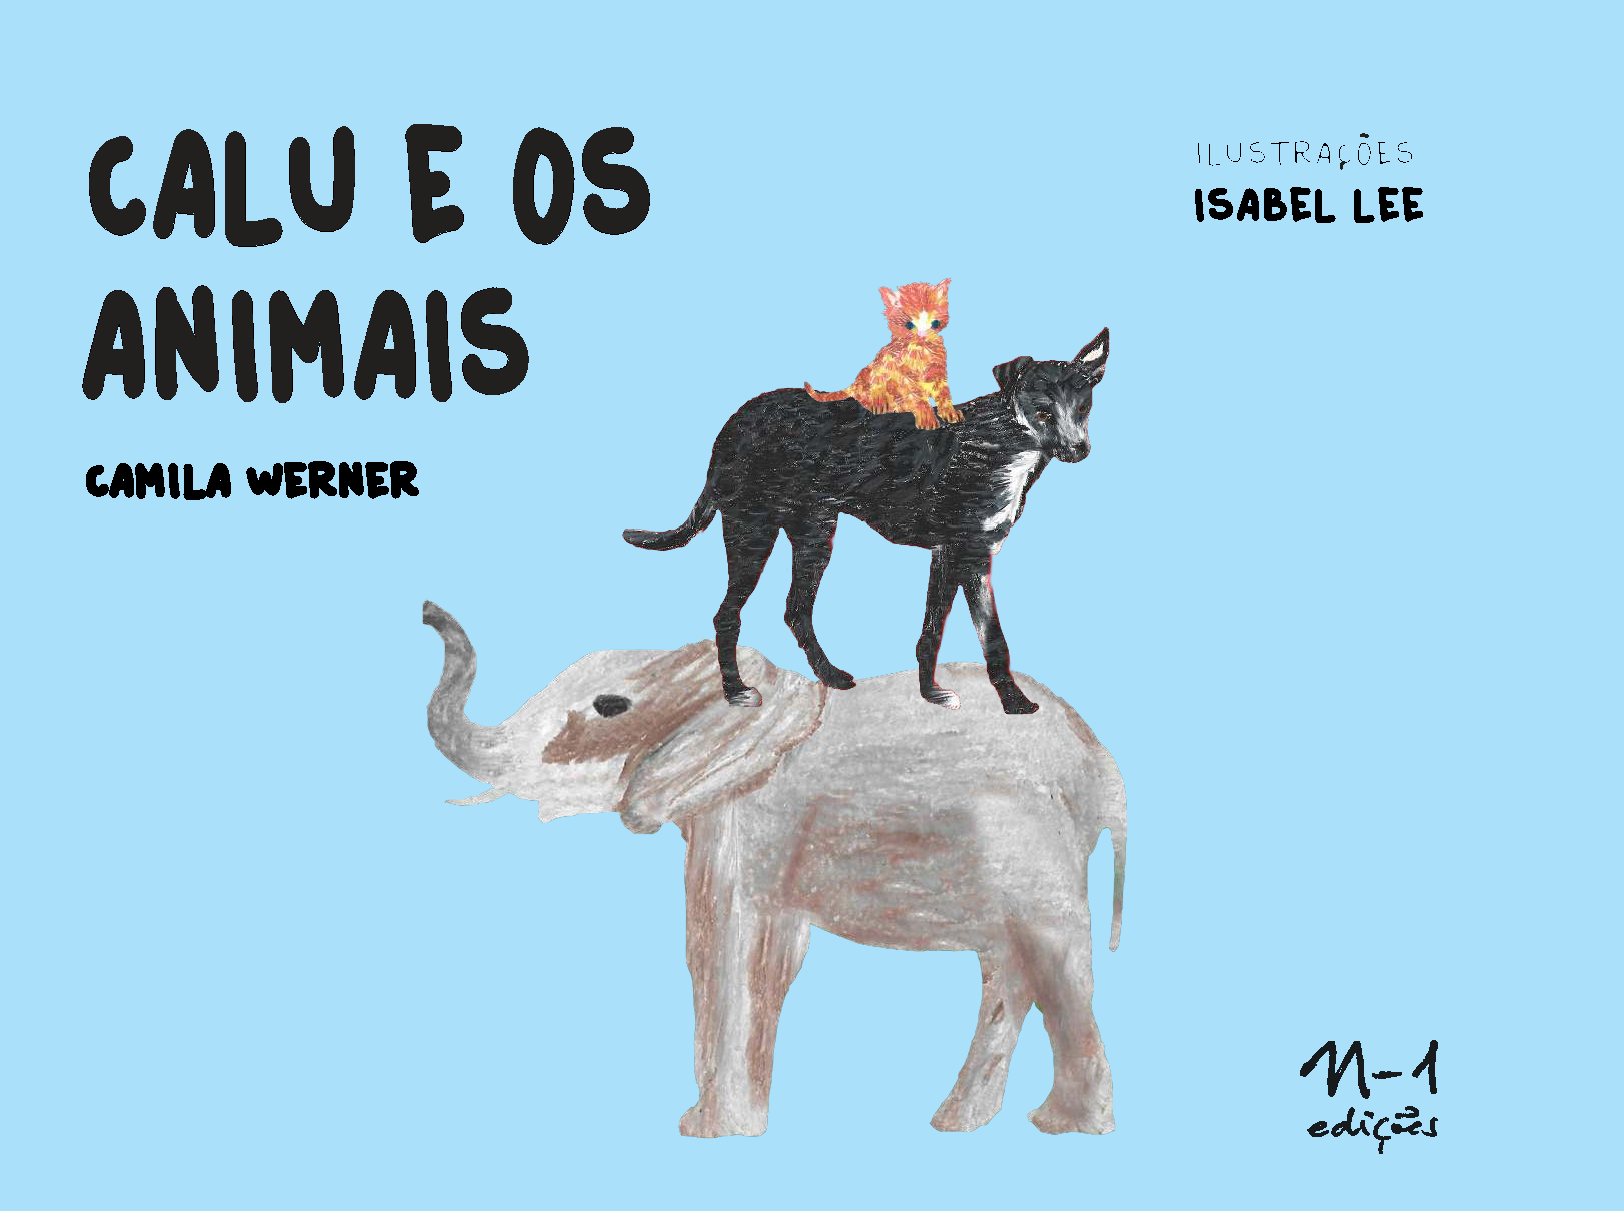
\includepdf[nup=2x2, 					% grid
			% offset=-15mm -5mm, 		% posição
			% scale=.8, 				% tamanho da página
            % delta=4mm 4mm, 			
            % frame,
            % pages={1-4}]{pdfs/PNLD2022-011_MIOLO.pdf}

\end{document}
